% --------------------- EMPIRICAL RESULTS -----------------------------
\section{Empirical Results}
\label{sec:results}

\subsection{Predictive performance}

Table~\ref{tab:acc} reports out-of-sample classification metrics across the nine model--horizon combinations and a naive benchmark that predicts $\hat{Y}_{i,t}=Y_{i,t-1}$. Three patterns stand out.

\begin{table}[H]
\centering
\small
\begin{tabular}{lccccccc}
\toprule
Model & Acc. & Prec. & Sens. & Spec. & F & AUROC & Pred.\ changes \\
\midrule
\texttt{index\_lag1} (naive) & 0.9507 & 0.9208 & 0.9399 & 0.9565 & 0.9303 & 0.9446 & 0 \\
\midrule
GLM-100  & 0.9506 & 0.9292 & 0.9328 & 0.9605 & 0.9310 & 0.9789 & 63  \\
GLM-60   & 0.9497 & 0.9293 & 0.9298 & 0.9607 & 0.9296 & 0.9808 & 76  \\
GLM-30   & 0.9482 & 0.9259 & 0.9288 & 0.9589 & 0.9274 & 0.9797 & 93  \\
XGBB-60  & 0.9408 & 0.9331 & 0.9043 & 0.9621 & 0.9184 & 0.9817 & 165 \\
XGBB-30  & 0.9398 & 0.9316 & 0.9030 & 0.9613 & 0.9171 & 0.9812 & 174 \\
XGBB-100 & 0.9380 & 0.9273 & 0.9025 & 0.9587 & 0.9148 & 0.9789 & 168 \\
XGBC-60  & 0.9317 & 0.9318 & 0.8834 & 0.9609 & 0.9069 & 0.9817 & 247 \\
XGBC-100 & 0.9266 & 0.9216 & 0.8795 & 0.9549 & 0.9000 & 0.9789 & 242 \\
XGBC-30  & 0.9260 & 0.9208 & 0.8780 & 0.9548 & 0.8989 & 0.9812 & 271 \\
\bottomrule
\end{tabular}
\caption{\textbf{Out-of-sample classification performance, 2010--2023.} Aggregated across 26 rebalancing events. The suffix denotes the prediction horizon in trading days before ED. \texttt{index\_lag1} is the trivial classifier that always predicts the previous-period label; XGBB is unconditional XGBoost; XGBC is XGBoost with the conditional posterior threshold of equation~(\ref{eq:cppt}). ``Pred.\ changes'' is the cumulative number of additions \emph{plus} deletions predicted across the test window.}
\label{tab:acc}
\end{table}

First, headline accuracy is genuinely high but is dominated by the trivial baseline: every learned model is statistically tied with simply repeating last period's label (95.07\%). Second, AUROC \parencite{fawcett-an-introduction-to-roc-analysis,hanley-area-under-a-receiver-operating-curve} tells a more useful story --- all models exceed 0.97, indicating that the ranking by $\hat{p}_{i,t}$ is informative even when the dichotomisation is not. Third, the conditional-threshold variant XGBC trades 1--2 percentage points of accuracy for a 60--70\% increase in the number of predicted changes (271 vs.\ 174 for the 30-day horizon), which is exactly the variable that determines whether the strategy can be \emph{traded}. The most accurate classifier in the table, \texttt{index\_lag1}, is the worst trader. This trade-off is the central methodological point of the paper.

\subsection{Active long--short strategy}

Table~\ref{tab:ff3} summarises the financial performance of the long--short overlay over 2010--2022, sorted by Sharpe ratio. OSEBX itself returned 0.95\% per month over the period at $\sigma=4.23\%$.

\begin{table}[H]
\centering
\small
\setlength{\tabcolsep}{4pt}
\begin{tabular}{lcccccccc}
\toprule
Portfolio & $R_p-R_b$ & $R_p$ & $\sigma_p$ & SR & $\alpha_{\text{CAPM}}$ & $\beta_{\text{MKT}}$ & TE$_{\text{ann}}$ & $\alpha_{\text{FF3}}$ \\
\midrule
OSEBX        & 0.0000  & 0.0095 & 0.0423 & 0.198 & 0.0002 & 1.015 & 0.000 & 0.001        \\
\midrule
GLM-60       & \textbf{0.0095}  & 0.0190 & 0.0756 & 0.237 & 0.0139 & 0.497 & 0.260 & \textbf{0.013$^{**}$} \\
GLM-30       & 0.0034  & 0.0129 & 0.0511 & 0.231 & 0.0048 & 0.863 & 0.126 & \textbf{0.006$^{**}$} \\
XGBC-30      & 0.0017  & 0.0112 & 0.0441 & 0.229 & 0.0026 & 0.925 & 0.079 & \textbf{0.004$^{**}$} \\
GLM-100      & 0.0087  & 0.0182 & 0.0757 & 0.226 & 0.0133 & 0.468 & 0.267 & \textbf{0.013$^{**}$} \\
XGBB-30      & 0.0010  & 0.0105 & 0.0488 & 0.192 & 0.0016 & 0.954 & 0.106 & 0.003        \\
XGBC-60      & $-$0.0029 & 0.0066 & 0.0480 & 0.114 & $-$0.0004 & 0.729 & 0.138 & 0.001 \\
XGBB-60      & $-$0.0019 & 0.0076 & 0.0608 & 0.107 &  0.0020 & 0.553 & 0.210 & 0.004 \\
\bottomrule
\end{tabular}
\caption{\textbf{Performance of long--short active overlays, monthly returns, January 2010 -- May 2022.} $R_p-R_b$ is the mean monthly excess return over OSEBX; SR is the Sharpe ratio against the Norwegian risk-free rate ($\approx$0.12\% per month); CAPM and FF3 alphas use OSEAX as the market proxy. Bold $\alpha_{\text{FF3}}$ entries are significant at the 5\% level (full FF3 regression in the appendix).}
\label{tab:ff3}
\end{table}

Four portfolios produce statistically significant Fama--French alpha at the 5\% level. They cluster into two economically distinct families. (i) The GLM portfolios are \emph{concentrated and volatile}: GLM-60 averages 1.9\% per month against $\sigma=7.6\%$, holds only 1--6 names per active window, and earns most of its alpha from a low market beta ($\beta=0.50$) rather than from raw return. (ii) The XGBC-30 portfolio is \emph{diversified and benchmark-like}: it places ten times as many trades per year, runs at $\beta=0.93$, has only 7.9\% annual tracking error against OSEBX, yet still produces a 0.4\% monthly FF3 alpha that is significant at 5\%. The fact that two qualitatively different portfolios both clear the FF3 hurdle is strong evidence that the predictability is real, not a single-strategy artifact. Figure~\ref{fig:cumret_active} plots the cumulative return paths of the four FF3-significant portfolios.

\begin{figure}[H]
\centering
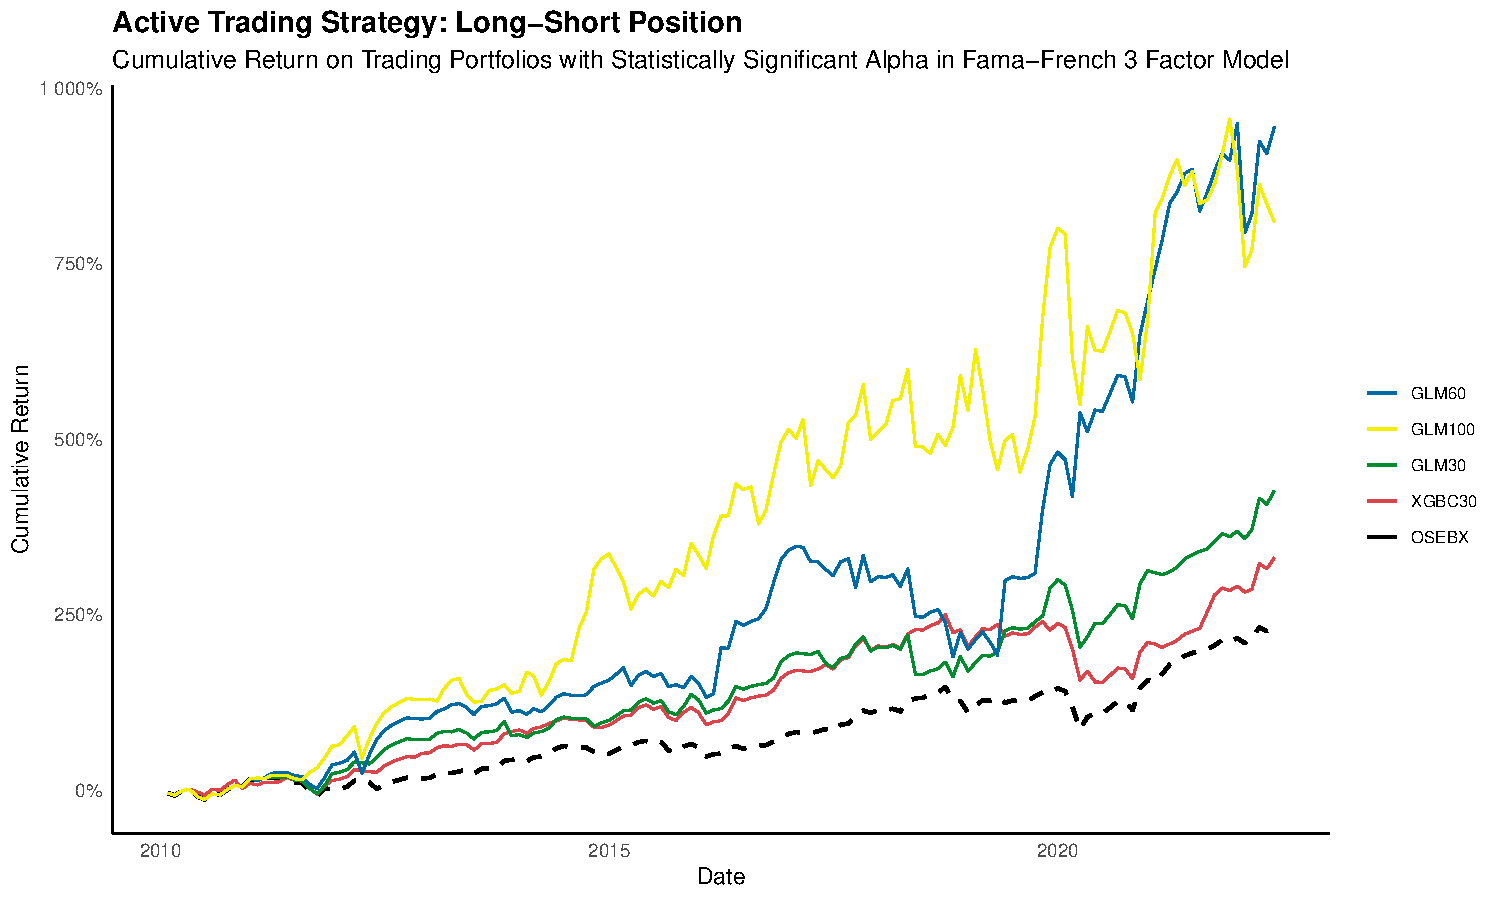
\includegraphics[width=0.85\linewidth]{images/trading_long_short.pdf}
\caption{\textbf{Cumulative returns, long--short active overlays vs.\ OSEBX, 2010--2023.} GLM-60 and GLM-100 are concentrated, high-volatility variants; XGBC-30 is the diversified variant produced by the conditional posterior-probability threshold of equation~(\ref{eq:cppt}). Initial capital is 1 NOK; transaction costs of 4 bps per leg and a 4\% short-borrow rate are applied.}
\label{fig:cumret_active}
\end{figure}

\subsection{Enhanced-index strategy}

When the active overlay is constrained to live inside a 2\% annual tracking error around OSEBX \parencite{ssg-tracking-error-enhanced}, the active weight $s$ in equation~(\ref{eq:enhanced}) varies sharply across portfolios: GLM-60's volatility limits it to a 4.1\% sleeve, while the lower-vol XGBC-30 can occupy 22.1\%. This rescaling reverses the active-overlay ordering. Figure~\ref{fig:cumret_enh} shows that all four enhanced portfolios track OSEBX tightly, but only XGBC-30 produces a positive Fama--French alpha that is statistically distinguishable from zero (0.0010 monthly, $p<0.10$).

\begin{figure}[H]
\centering
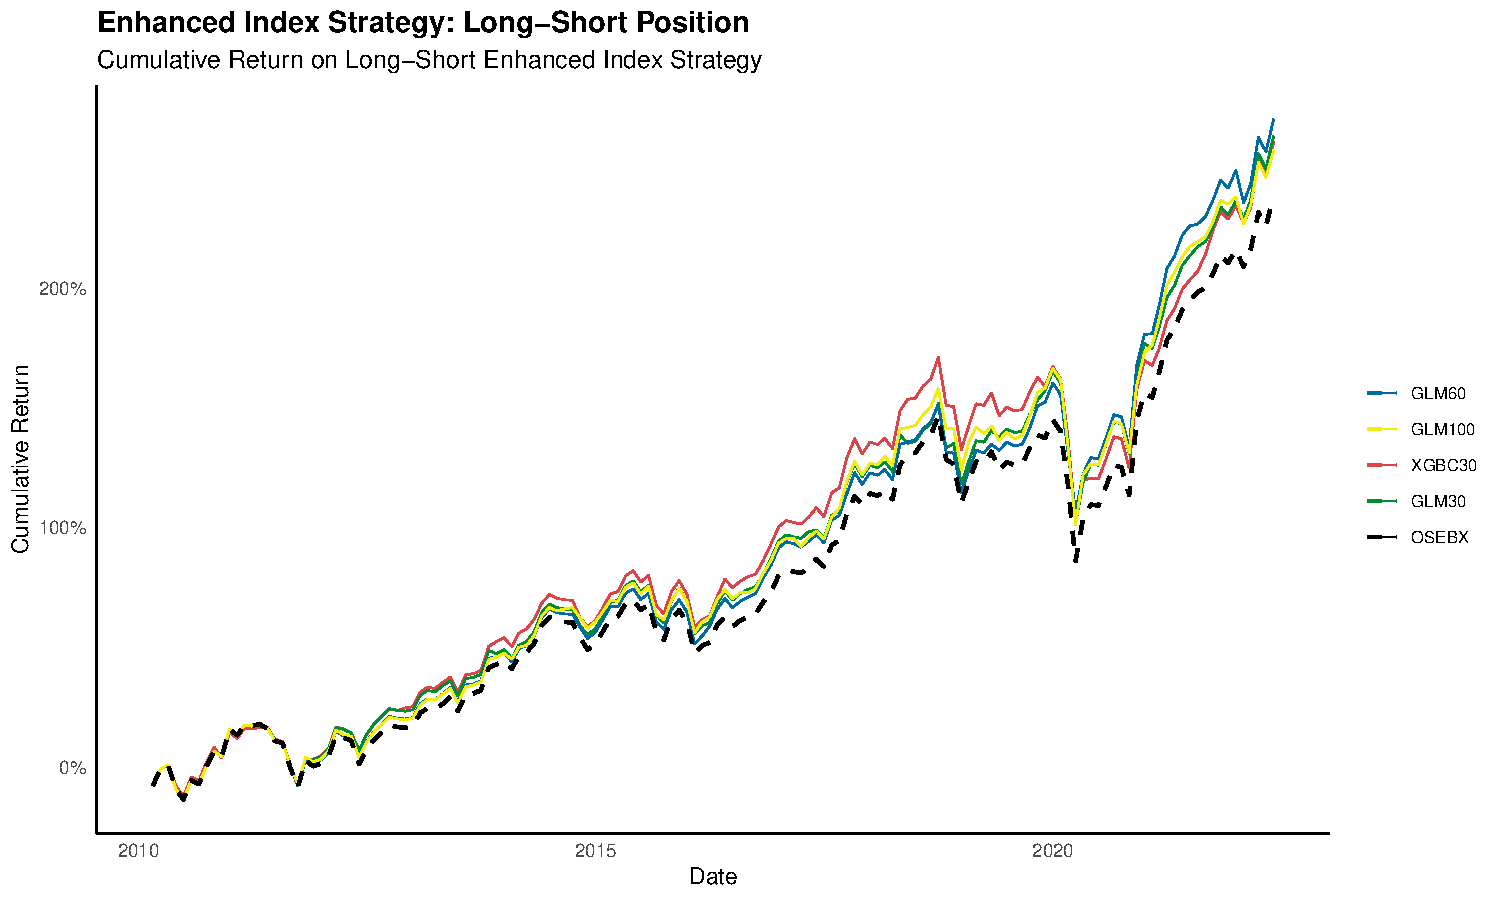
\includegraphics[width=0.85\linewidth]{images/enhanced_long_short.pdf}
\caption{\textbf{Cumulative returns, enhanced-index portfolios vs.\ OSEBX, 2010--2023.} Each portfolio combines its long--short active overlay with a passive OSEBX sleeve, with the active weight chosen to deliver a 2\% annual tracking error. The XGBC-30 enhanced portfolio produces a Fama--French alpha significant at the 10\% level; the GLM-based variants do not, despite outperforming on raw return, because their concentration forces a tiny active sleeve.}
\label{fig:cumret_enh}
\end{figure}

The economic interpretation is the practical lesson of the paper. In an unconstrained active mandate, concentrated GLM forecasts win on raw alpha. In a tracking-error-constrained enhanced-index mandate --- which is the actual product DNB and other Nordic asset managers are launching \parencite{dnb-global-enhanced-index,jp-morgan-enhanced-index} --- the diversified, deliberately-less-accurate XGBC-30 is the only forecast that survives risk adjustment. The conditional posterior threshold of equation~(\ref{eq:cppt}) was designed precisely to manufacture that diversification, by trading classification accuracy for signal count.
